\documentclass[10pt,a4paper]{article}
\usepackage[utf8]{inputenc}
\usepackage[T1]{fontenc}
\usepackage[french]{babel}
\usepackage{booktabs,graphicx,geometry,hyperref,xcolor,amsmath,amssymb,array}
\usepackage{pdflscape,longtable,float,caption,titlesec}
\geometry{margin=1.6cm}
\usepackage{url}\urlstyle{tt}
\hypersetup{colorlinks=true,linkcolor=blue!45!black,citecolor=blue!45!black}
\captionsetup{font=small,labelfont=bf}
\setcounter{topnumber}{3}\setcounter{bottomnumber}{2}
\setcounter{totalnumber}{5}
\renewcommand{\topfraction}{0.92}
\renewcommand{\bottomfraction}{0.75}
\renewcommand{\textfraction}{0.06}
\renewcommand{\floatpagefraction}{0.75}
\setlength{\parskip}{3pt}

\titleformat{\section}{\large\bfseries}{\thesection}{0.8em}{}
\renewcommand{\arraystretch}{1.05}

\title{\huge\textbf{Analyse des résultats}\\[4pt]
\large Arctic-TVC — ce que disent les 42 modèles, et ce que ça change\\[6pt]
\normalsize Document d'interprétation — le compagnon du \texttt{compendium.pdf}
(qui, lui, s'interdit d'interpréter)}
\date{\today}

\begin{document}
\maketitle

\begin{abstract}
\noindent Le compendium rassemble les mesures ; ce document les lit. Sept constats,
dans l'ordre où ils s'imposent :
\textbf{(1)}~l'adaptation d'un backbone fonctionne (LoRA r=8 bat son gelé de
+0,0114, $p=0{,}0012$), mais aucun modèle déployable ne dépasse le meilleur gelé ;
\textbf{(2)}~sur SimDINOv2-B, le paysage de l'adaptation est plat (13~bras dans
0,0067, NormTuning = LoRA au millième près avec $\approx$47k paramètres) ;
\textbf{(3)}~le scaling LoRA dégrade partout et l'hypothèse rsLoRA est infirmée ;
\textbf{(4)}~le contexte spatial est le plus grand levier mesuré (+0,025 à +0,034),
validé par contrôles apparié et permuté ;
\textbf{(5)}~le pré-entraînement aligné (iNat-Plantae) compte plus que l'échelle et
que l'adaptation : gelé-fusionné à 0,5059 sans entraînement ;
\textbf{(6)}~avec un palier élargi à 35~modèles, la séparabilité des classes ordonne
significativement les modèles (le verdict « artefact » à $n=14$ était un manque de
puissance) tandis que la famille spectrale reste anti-prédictive ;
\textbf{(7)}~au sommet du plateau, le choix de la régularisation $C$ pèse autant
que le choix du bras ($\pm$0,0074 sur un seed).
Chaque constat renvoie aux tableaux et figures du compendium ; aucun chiffre n'est
saisi à la main ici non plus.
\end{abstract}

\tableofcontents
\newpage

% ════════════════════════════════════════════════════════════
\section{Le benchmark : 42 modèles, un palier à 35}\label{ana:bench}
% ════════════════════════════════════════════════════════════

Le tableau maître compte 42~modèles (11~gelés, 29~affinés à 3~seeds, 2~bornes
fusionnées non déployables), tous évalués par le même probe canonique sur le même
test (17\,598~tuiles). Le palier compétitif — fixé par la rupture mesurée du
classement, pas par une coupe de rang — contient 35~modèles (0,5080 à 0,4689,
décrochage de +0,0069 au rang suivant). Le bootstrap apparié hiérarchique couvre
33~groupes (528~paires, 108 rejetées par Benjamini-Hochberg) ; les 2~bornes
SimDINOv2-B entraînées, sans embeddings rapatriés, restent des point-estimates
documentés.

\begin{figure}[htbp]
\centering
\includegraphics[width=0.90\textwidth]{figs/perf_ranking_ci.png}
\caption{Le classement complet. Deux choses se voient sans statistique : la tête
détachée (R2, borne fusionnée non déployable) et le ventre mou du milieu de
palier, où une douzaine de régimes d'adaptation se tiennent dans 0,01.}
\end{figure}

\begin{landscape}
\small
\input{tables/t_master}
\end{landscape}

% ════════════════════════════════════════════════════════════
\section{L'adaptation est bornée}\label{ana:bounded}
% ════════════════════════════════════════════════════════════

Le premier résultat tient en deux tableaux. Sur DINOv3-B, seul LoRA r=8 bat
significativement son propre backbone gelé (+0,0114, $p=0{,}0012$) ; Full et MHSA
n'y arrivent pas après correction. Mais LoRA r=8 contre DINOv3-L gelé donne
$\Delta=+0{,}0038$, $p=0{,}39$ : \textbf{l'adaptation rattrape la capacité, elle ne
la dépasse pas}. Le même schéma se répète sur SimDINOv2-B avec une nuance
intéressante : les bras parcimonieux (b911, b611) et NormTuning battent le gelé
($p\leq0{,}0043$) quand le LoRA complet tous blocs n'y arrive pas ($p=0{,}058$).
Adapter moins, mais au bon endroit, vaut mieux qu'adapter partout.

\input{tables/t_dinov3b_regimes}

\input{tables/t_simb_regimes}

\noindent\textbf{Échelle contre adaptation.} DINOv3-B + LoRA r=8 (86,3M paramètres
dont 0,295M entraînables) égale le meilleur F1 du benchmark face à DINOv3-H+ gelé
(840M) : le rapport F1/paramètres est $\approx$10 fois supérieur côté adaptation.
Mais un ViT-S LoRA (22M) bat aussi le ViT-B gelé (86M) : à l'intérieur d'une
famille, l'adaptation rapporte ce que l'échelle rapporte. Ni l'une ni l'autre ne
change l'ordre de grandeur — seule l'information (section~\ref{ana:ctx}) le fait.

\input{tables/t_cost_perf}

\begin{figure}[htbp]
\centering
\includegraphics[width=\textwidth]{figs/cost_perf.png}
\caption{F1 contre coût, échelle log. L'adaptation est l'option efficace à budget
fixé ; elle ne déplace pas le plafond.}
\end{figure}

% ════════════════════════════════════════════════════════════
\section{Le paysage PEFT est plat}\label{ana:plateau}
% ════════════════════════════════════════════════════════════

Treize bras $\times$ 3~seeds sur SimDINOv2-B (position, rang 2 à 32, scaling 1 à 4,
Q+K+V, rsLoRA, NormTuning), même test, F1 canonique : \textbf{tout tient dans
0,0067}. Aucun rang, aucun $\alpha$, aucun type ne bat l'ancre r8a8 tous blocs
(0,4781) au-delà du bruit inter-seed.

\input{tables/t_simb_ablation}

\paragraph{Rang.} Pente douce décroissante (r2 : 0,4793 $\to$ r32 : 0,4750), pas de
falaise comme sur DINOv3-B. Le rang 8 du manuscrit est sur un plateau, pas à un
optimum.

\begin{figure}[htbp]
\centering
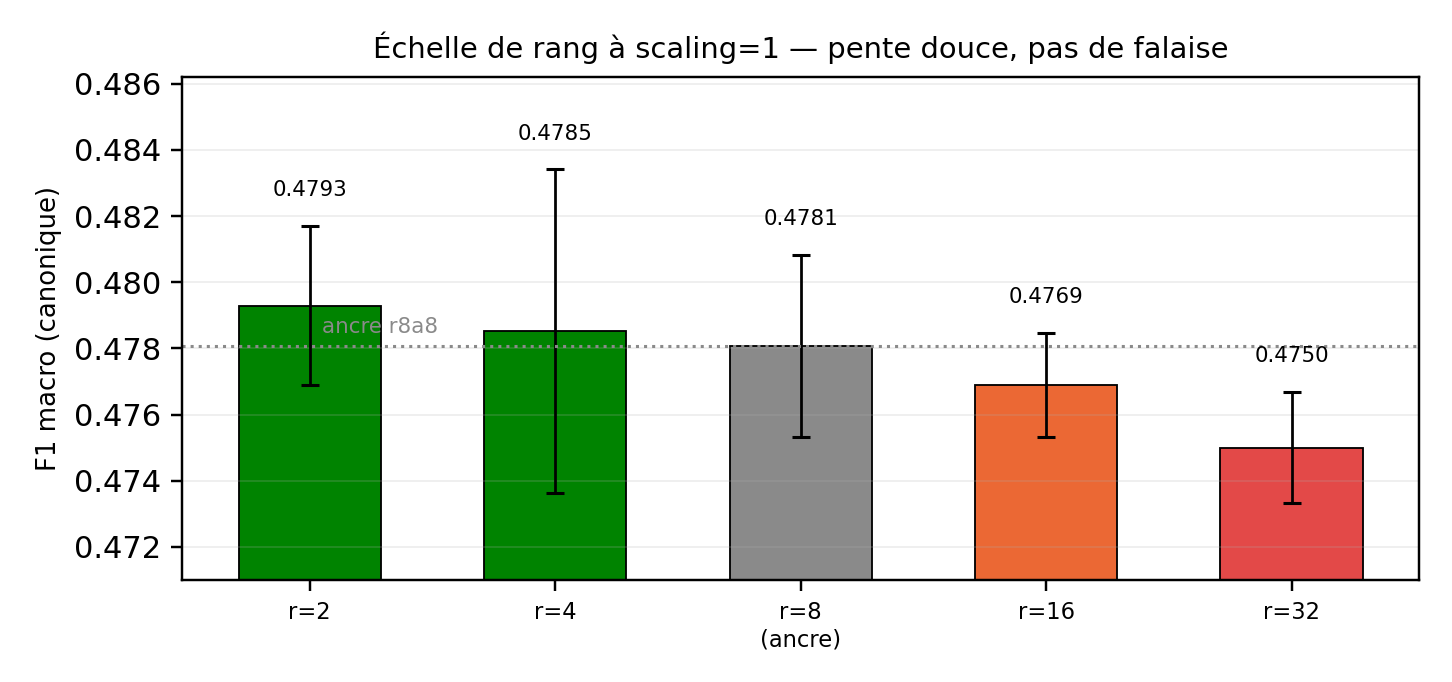
\includegraphics[width=0.72\textwidth]{figs/peft_rank_ladder.png}
\caption{Échelle de rang à scaling=1. La pente existe mais reste sous le seuil
d'interprétabilité entre voisins.}
\end{figure}

\paragraph{Scaling : rsLoRA infirmé.} À r=8 comme à r=16, plus de scaling = pire,
de façon monotone (0,4781 $\to$ 0,4760 $\to$ 0,4753 ; 0,4769 $\to$ 0,4749 $\to$
0,4737). L'hypothèse rsLoRA (le scaling devrait croître en $\sqrt{r}$) prédit
l'inverse de ce qui est mesuré. Corollaire : le décrochage r=16/32 observé sur
DINOv3-B n'était pas un artefact de scaling — c'est un effet de rang réel.
Convention $\alpha=r$ validée.

\begin{figure}[htbp]
\centering
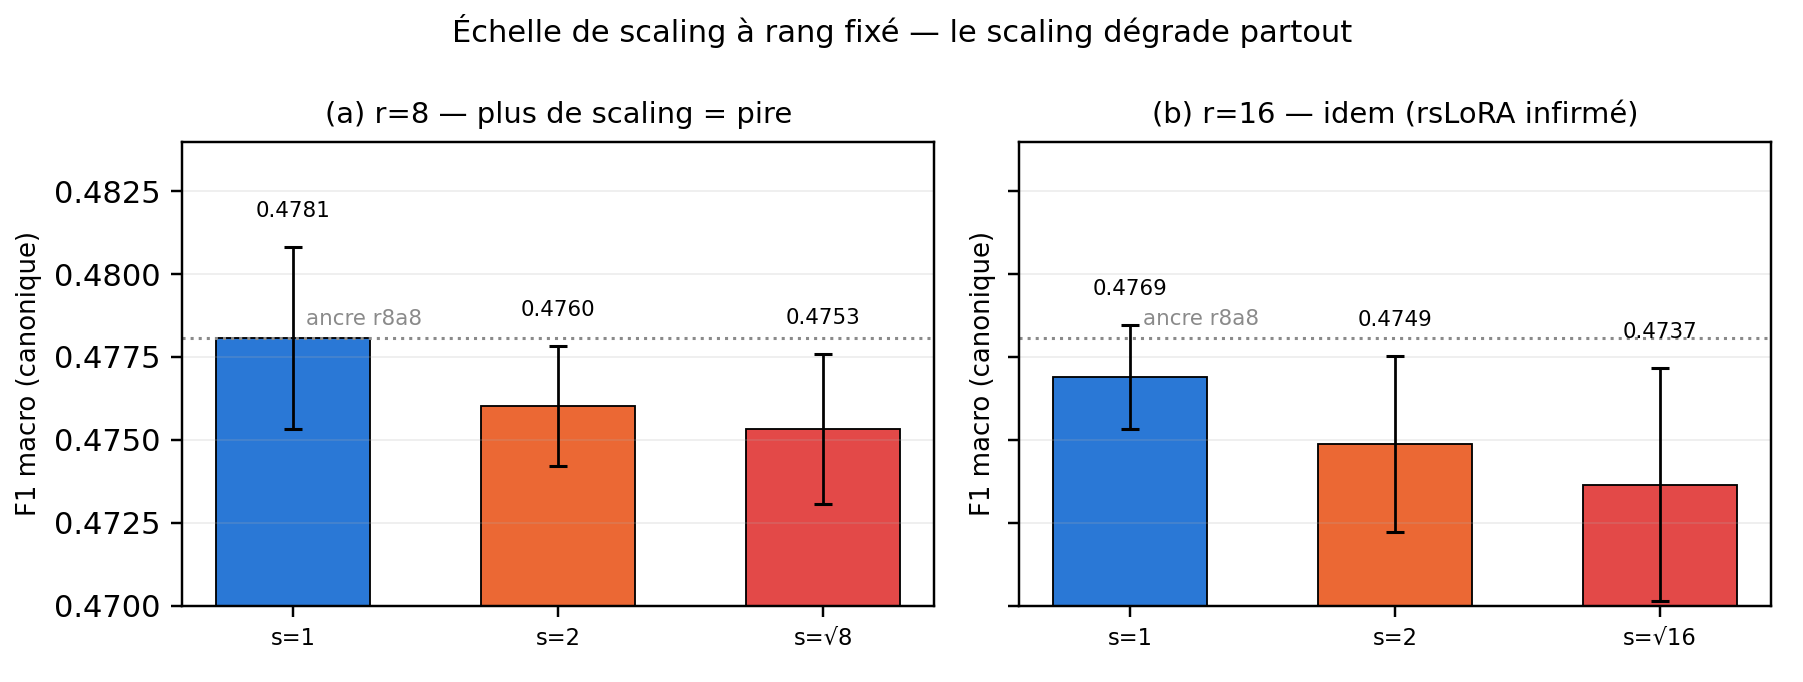
\includegraphics[width=0.92\textwidth]{figs/peft_scaling_ladder.png}
\caption{Échelle de scaling à rang fixé. Les deux panneaux disent la même chose :
le scaling dégrade, monotone.}
\end{figure}

\paragraph{Position et type.} L'ordre DINOv3 se transpose : blocs hauts $\geq$ tous
blocs $\gg$ blocs bas. Le bras b911 (3~derniers blocs, un quart du budget du LoRA
complet) est le plus stable du job ($\pm$0,0002). Ajouter K aux cibles (Q+K+V)
rapporte +0,0007 : rien de mesurable.

\begin{figure}[htbp]
\centering
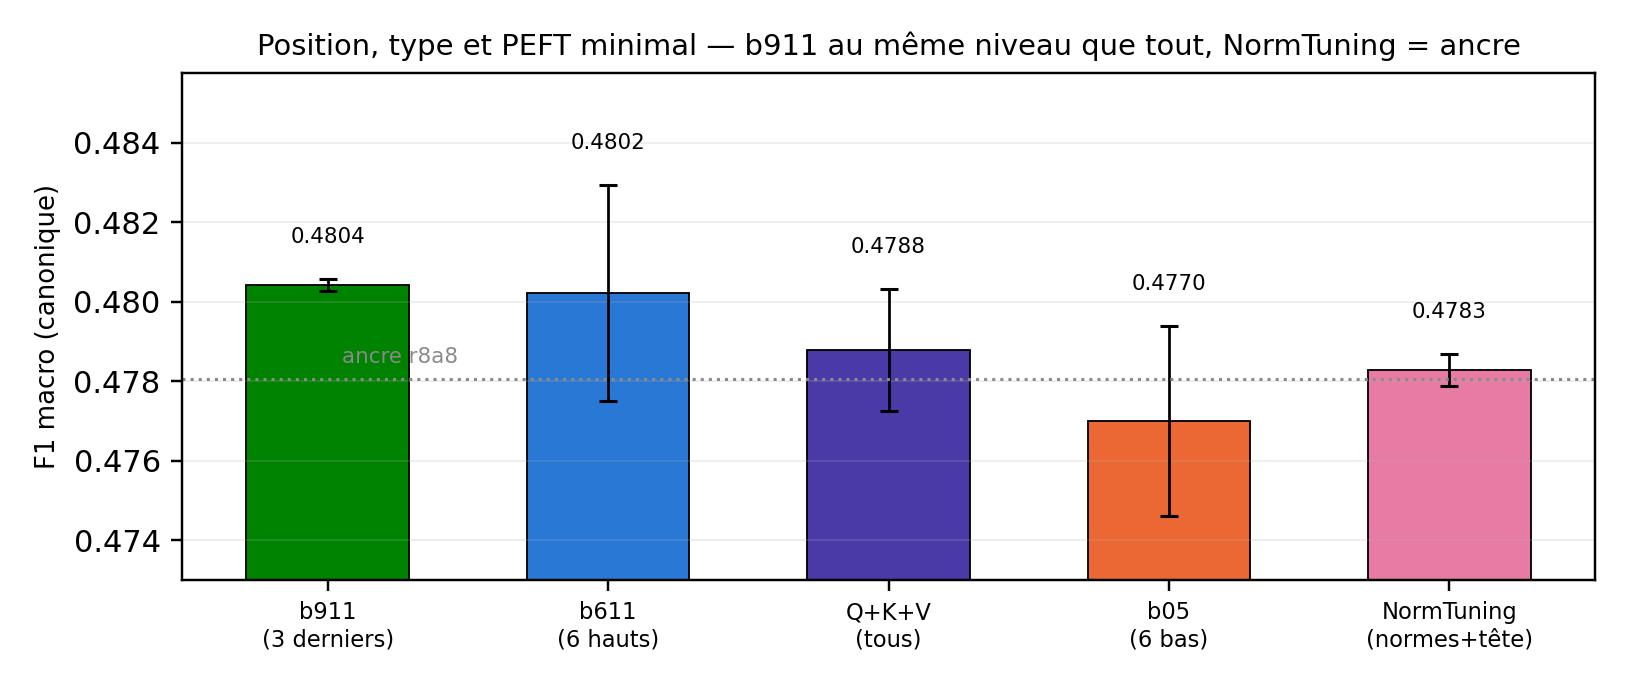
\includegraphics[width=0.80\textwidth]{figs/peft_position.png}
\caption{Position, type, PEFT minimal. b911 fait aussi bien que tout avec un quart
du budget ; NormTuning égale l'ancre.}
\end{figure}

\paragraph{NormTuning = LoRA.} C'est le résultat structurel de la campagne :
0,4783 $\pm$ 0,0004 contre 0,4781 $\pm$ 0,0028 pour l'ancre ($\Delta=+0{,}0002$,
$p=0{,}94$ au bootstrap — indistinguables), avec $\approx$47k paramètres (normes +
tête, aucun adaptateur). \textbf{LoRA n'apporte rien qu'une mise à jour des normes
ne donne déjà} sur ce backbone. Côté géométrie pourtant, les deux chemins
diffèrent : NormTuning contracte le rang à mi-chemin du LoRA (68,4 contre 58,1,
gelé 86,3) — même F1, chemin géométrique différent.

\paragraph{Caveat de sélection du C.} Au sommet du plateau, le choix de la
régularisation pèse autant que le choix du bras : le run QKV seed2 vaut 0,4873 à
$C=0{,}0001$ (probe interne) contre 0,4799 à $C=0{,}001$ (canonique), soit
$\pm$0,0074 par basculement de $C$. La valeur canonique est retenue partout ; les
écarts entre conventions sont tracés, pas cachés.

\paragraph{DINOv3-B : rang et blocs (rappel).} L'ablation du rang (plateau r=2/4/8,
décroissance à 16/32) et l'ablation de blocs (6~hauts $\geq$ 12, 6~bas au niveau
Full) fondent la recette r=2--8 sur blocs hauts reprise sur SimB.

\input{tables/t_lora_rank}

\begin{figure}[htbp]
\centering
\includegraphics[width=0.9\textwidth]{figs/lora_rank_curve.png}
\caption{Ablation du rang, DINOv3-B : le plateau puis la décroissance.}
\end{figure}

\input{tables/t_lora_block_ablation}

% ════════════════════════════════════════════════════════════
\section{Le contexte : le vrai levier}\label{ana:ctx}
% ════════════════════════════════════════════════════════════

Le contexte spatial (fenêtre 512--1024px autour de la tuile) apporte +0,025 à
+0,034 de F1 — deux à trois fois le meilleur gain d'affinage mesuré dans ce projet.
Mais à trois conditions, établies par les contrôles : appariement spatial exact,
exploitation apprise ou pré-alignée, et taille modérée (512 $>$ 1024 $\gg$ 2048,
le 2048 lissé par le redimensionnement n'apporte rien).

\paragraph{Distillation seule : rien. Fusion apprise : +0,021.} Le design A
(contexte au train seulement) ne bat pas les baselines LoRA (0,4870 contre
0,4835--0,4844, dans le bruit) ; le teacher externe n'apporte rien face à l'EMA
self (+0,003). Le design B (tête apprise sur la fusion) explose à 0,5080 — et son
backbone devient le \emph{pire} en tuile seule (0,4779) : l'entraînement B
réorganise le réseau pour dépendre du contexte.

\input{tables/t_ctx_distill}

\begin{figure}[htbp]
\centering
\includegraphics[width=0.80\textwidth]{figs/fig_ctx_f1.png}
\caption{F1 par design. Les deux SimDINOv2-B @512 entraînés plafonnent au niveau
du gelé-fusionné : entraîner la fusion n'apprend rien de plus que la sonde quand
le pré-entraînement est aligné.}
\end{figure}

\input{tables/t_ctx_matrix}

\begin{figure}[htbp]
\centering

\includegraphics[width=0.72\textwidth]{figs/fig_ctx_matrix.png}
\caption{Le contexte aide tout le monde ; seul R2 franchit 0,51, au prix d'une
tuile seule dégradée.}
\end{figure}

\paragraph{Contrôles Bouguessa : le gain est spatial.} Contexte seul = tuile seule
(0,4781 contre 0,4778) : la fenêtre voisine porte autant d'information que la
tuile centrale. Contexte permuté = \emph{sous} la tuile seule (0,4745) : une
seconde représentation désalignée dégrade — le gain vient de l'appariement
spatial, pas de la concaténation.

\input{tables/t_ctx_controls}

\paragraph{Le pré-entraînement compte plus que l'échelle et l'adaptation.}
SimDINOv2-B (iNat-Plantae) gelé-fusionné à 0,5059, \emph{sans aucun entraînement},
égale presque R2 entraîné (0,5080) et bat toute la famille DINOv3 frozen-fusionnée
à toutes les tailles. SimDINOv2-L (300M, même pré-entraînement) n'ajoute rien
(0,5022) : c'est l'alignement du pré-entraînement qui porte le décodage du
voisinage, pas la taille.

\input{tables/t_ctx_sweep}

\begin{figure}[htbp]
\centering
\includegraphics[width=0.66\textwidth]{figs/fig_ctx_geom.png}
\caption{Le fine-tuning déplie l'espace latent ; la branche tuile-seule de R2
reste anisotrope — le backbone B s'appuie sur le contexte.}
\end{figure}

% ════════════════════════════════════════════════════════════
\section{Géométrie : ce qui ordonne, ce qui n'ordonne pas}\label{ana:geom}
% ════════════════════════════════════════════════════════════

\paragraph{Famille DINOv3-B : F1 constant, géométries séparées.} Le gelé et ses
régimes tiennent dans une bande de F1 étroite pendant que l'anisotropie et le rang
effectif varient d'un facteur plusieurs : la géométrie distingue des modèles que
le F1 ne distingue pas — sans pour autant les classer (voir ci-dessous).

\input{tables/t_family}

\begin{figure}[htbp]
\centering
\includegraphics[width=\textwidth]{figs/geom_dinov3b_family.png}
\caption{Coordonnées parallèles : même F1 à $\pm$0,012 près, géométries nettement
séparées.}
\end{figure}

\paragraph{Peut-on classer les meilleurs ? Oui, avec la séparabilité — à
condition d'avoir assez de modèles.} C'est le résultat qui a changé cette nuit :
sur le palier à 14, aucune métrique ne passait le seuil (IC95 traversant zéro
partout) ; sur le palier à 35, peuplé par les 13~bras d'adaptation graduée, la
famille séparabilité passe la correction BH (Fisher 411/592 paires, $p=0{,}013$ ;
CHI et NC1 $p=0{,}014$ ; DBI $p=0{,}039$ ; silhouette $p=0{,}026$ en paires). Sa
\emph{direction} était stable sur tous les paliers restreints testés : l'effet
existe, $n=14$ ne donnait pas la puissance pour le déclarer. La famille spectrale,
elle, reste anti-prédictive (41--42~\% des paires) et ne redevient positive que
sur la population complète : sa corrélation d'ensemble est portée par les modèles
cassés. Seule la pureté k-NN désigne le vrai n\textsuperscript{o}~1 (R2).

\input{tables/t_tier_ranking}

\begin{figure}[htbp]
\centering
\includegraphics[width=\textwidth]{figs/geom_tier_ranking.png}
\caption{(a) Le signe dépend de la population. (b) Pouvoir d'ordonnancement sur le
palier de 35. (c) La séparabilité forme un bloc unique.}
\end{figure}

\input{tables/t_tier_signs}

\begin{figure}[htbp]
\centering
\includegraphics[width=0.90\textwidth]{figs/geom_corr_forest.png}
\caption{Corrélations de Spearman par population : la séparabilité ne devient
significative que sur le palier peuplé.}
\end{figure}

% ════════════════════════════════════════════════════════════
\section{Significativité : ce qui survit à Benjamini-Hochberg}\label{ana:signif}
% ════════════════════════════════════════════════════════════

Sur les 528~paires testées, 108 sont rejetées. Les verdicts qui comptent :

\begin{itemize}
\item LoRA r=8 bat son gelé (+0,0114, $p=0{,}0012$) ; MHSA ($p=0{,}016$) et Full
($p=0{,}101$) ne passent plus la correction sur 528 paires.
\item b911, b611 et NormTuning battent le gelé SimB ($p\leq0{,}0043$) ; le r8a8
tous blocs n'y arrive pas ($p=0{,}058$).
\item R2 bat tout le monde ($+0{,}025$ à $+0{,}029$, $p<10^{-4}$) — borne non
déployable, pas modèle.
\item Aucun modèle déployable ne dépasse le meilleur gelé (LoRA r=8 contre
DINOv3-L : $p=0{,}39$ ; b911 contre DINOv3-L : $p=0{,}64$).
\item NormTuning contre ancre LoRA : $p=0{,}94$. b911 contre b05 : $p=0{,}23$.
Le plateau est statistiquement un plateau.
\end{itemize}

\input{tables/t_ci}

\input{tables/t_signif_bh}

\begin{figure}[htbp]
\centering
\includegraphics[width=\textwidth]{figs/perf_signif_matrix.png}
\caption{Matrice de significativité, 33~groupes. Les blocs de non-rejet au centre
sont le palier plat SimDINOv2-B.}
\end{figure}

% ════════════════════════════════════════════════════════════
\section{Ce que ça veut dire pour le mémoire}\label{ana:thesis}
% ════════════════════════════════════════════════════════════

\begin{enumerate}
\item \textbf{Le message en une phrase} : sur Arctic-TVC, ce qui compte n'est pas
la capacité paramétrique ajoutée (adaptation ou échelle) mais l'information donnée
au modèle — pré-entraînement aligné au domaine et voisinage spatial de la tuile.
\item \textbf{Le fine-tuning n'est pas inutile} (LoRA bat son gelé, $p=0{,}0012$),
mais son rendement est borné : il rattrape la capacité, ne la dépasse pas. Le
dire ainsi évite à la fois le « l'adaptation ne sert à rien » (faux) et le
« l'adaptation suffit » (faux aussi).
\item \textbf{Le chapitre PEFT} (rang, blocs, Stage A, NormTuning, rsLoRA) est le
plus original du mémoire : personne dans le corpus ne fait d'ablation
r$\times\alpha\times$position sur FM géospatiales, et le résultat est négatif de
façon informative (plafond informationnel, pas échec de tuning).
\item \textbf{Le chapitre géométrie} doit raconter la révision : direction stable,
seuil franchi à $n=35$ — un exemple propre de raisonnement en puissance
statistique, et une mise en garde contre les conclusions à petit $n$.
\item \textbf{Le chapitre contexte} porte le chiffre le plus fort (+0,03) avec les
contrôles les plus propres (appariement, permutation, sweep de tailles) : c'est
lui qui mérite la discussion la plus longue.
\item \textbf{Les caveats à garder} : sélection du $C$ au sommet du plateau,
divergence val/test pour la sélection de bras, R2 et SimB entraînés non
déployables, 2~bornes SimB en point-estimates (pas d'embeddings rapatriés).
\end{enumerate}

\end{document}
